All coefficient and count checks pass. The 480-fit grid reproduces
full-information regret within $3.81\times10^{-12}$ in all 80 pairs.
All 120 additional checkpoints pass independent re-evaluation; the
110 exact-recovery/full-information comparisons differ in regret by
at most $8.04\times10^{-13}$ and in closed-loop cost by
$2.83\times10^{-11}$. The maximum coefficient error across all direct
checks is $3.56\times10^{-15}$. This is the expected consequence of
preserving the objective, not evidence of a better optimizer.

Every random-embedding cache has $r=\min(k,m)$. In the box caches,
relevant, hybrid and pruned hybrid each use 332,362 responses; student
basis and its orthogonal rotation use 444,234; full face uses 1,039,456.
Thus the 68.03\% reduction against full-face recovery is shared by the
simple hybrid. Relevant queries save 25.18\% against the direct student
basis and \emph{nothing against hybrid}. Ball counts likewise match
hybrid. The ambient-random baseline's failures do not extend to a
complete orthogonal student-space basis.

In the shared-actuation construction, all 61,440 cached states have
$k=3,m=4,r=1$. Relevant feedback uses one query per state, hybrid and
pruned hybrid three, and either student basis four
(Figure~\ref{fig:direct-query}). Every recovery method yields mean
regret 0.523674 and mean closed-loop cost 189.698903, versus 0.627840
and 190.883229 for target-only fitting. The extra saving depends on
linear dependence among visible directions, not simply zero-coordinate
pruning. The construction establishes this possibility, not its
prevalence in applications.
\begin{figure}[htbp]\centering
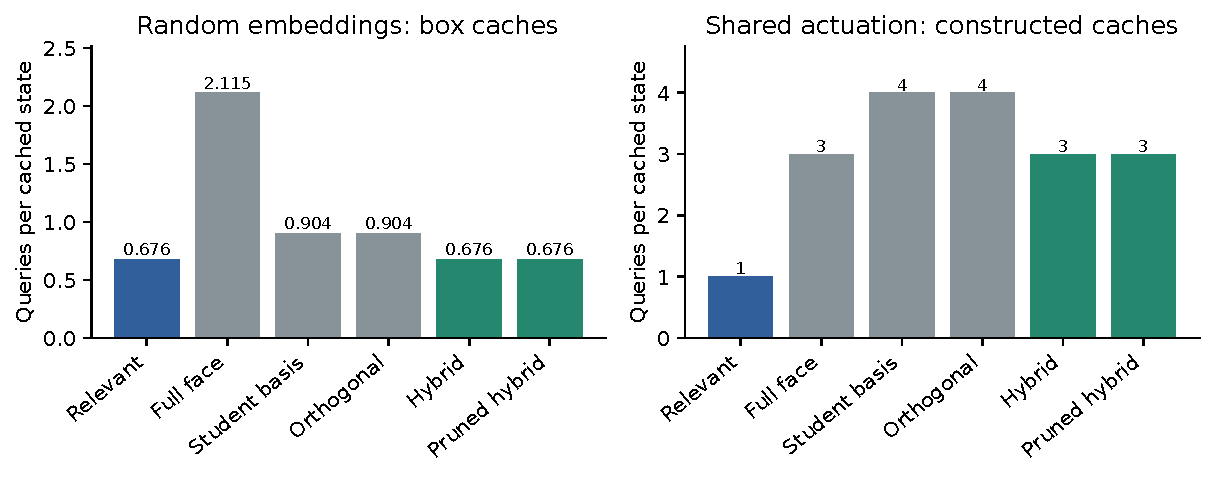
\includegraphics[width=\linewidth]{figures/direct_query_controls.pdf}
\caption{Direct controls separate dimension reduction from additional
alignment. Counts include inactive targets. Left: all random-embedding
box caches; relevant and hybrid coincide. Right: a constructed shared
actuation geometry; every state has positive rank one.}
\label{fig:direct-query}
\end{figure}
\begin{table}[htbp]\centering\small
\caption{Additional interface checks: means over five paired seeds. All exact-recovery interfaces agree to the reported precision; full-reference values are shown. These checks reuse four conditions and add a constructed shared-actuation condition.}\label{tab:direct-training}
\begin{tabular}{lrrrr}\toprule
Condition & Fits & Regret & Cost & Max. $|\Delta\mathcal R|$\\\midrule
box, $d=8,m=2,R=0.5$ & 20 & 0.585439 & 8.101119 & $0$\\
box, $d=32,m=2,R=0.5$ & 20 & 0.900619 & 15.475675 & $0$\\
box, $d=32,m=4,R=2$ & 20 & 0.820332 & 15.014408 & $0$\\
ball, $d=32,m=4,R=0.5$ & 20 & 0.715371 & 15.313708 & $8.03\times10^{-13}$\\
Shared actuation & 40 & 0.523674 & 189.698903 & $0$\\
\bottomrule\end{tabular}
\end{table}


Timing includes geometry, query construction, actual responses and
decoding on 12,288-state batches, after one warmup and with three
shuffled repeats. Median batch times on random box caches are 1.348\,ms
for relevant, 0.753\,ms for student basis and 0.890\,ms for hybrid;
on structured caches they are 2.268, 0.879 and 0.802\,ms. With this cheap
analytic oracle, rank construction costs more than the saved responses.
These implementation measurements do not support a runtime advantage.

The complete grid, including gain/random failures and uncertain
target-only comparisons, is in \ref{app:minimal-grid} and
\ref{app:minimal-comparisons}. A further 2,304 algebraic checks verify
Eq.~\eqref{eq:truncated-feedback}: arbitrarily small perturbations can
raise exact rank from one to three, while one-query approximation error
changes continuously with the omitted singular values
(\ref{app:approximate-feedback}). No noisy neural training is claimed.
